% Math Class Notes
% Prepared by Chen Gao
% SPDX-License-Identifier: MIT

\documentclass[12pt,a4paper]{article}

% Copyright (c) Brandon Pacewic
% SPDX-License-Identifier: MIT

% Fix section numbering
\setcounter{secnumdepth}{3}
\renewcommand{\thesection}{\arabic{section}}
\renewcommand{\thesubsection}{\thesection.\arabic{subsection}}

\usepackage[tmargin=2cm,rmargin=1in,lmargin=1in,margin=0.85in,bmargin=2cm,footskip=.2in]{geometry}
\usepackage{amsmath,amsfonts,amsthm,amssymb,mathtools}
\usepackage[varbb]{newpxmath}
\usepackage{xfrac}
\usepackage[makeroom]{cancel}
\usepackage{mathtools}
\usepackage{bookmark}
\usepackage{enumitem}
\usepackage{hyperref,theoremref}
\hypersetup{
	pdftitle={Assignment},
	colorlinks=true, linkcolor=doc!90,
	bookmarksnumbered=true,
	bookmarksopen=true
}
\usepackage[most,many,breakable]{tcolorbox}
\usepackage{xcolor}
\usepackage{varwidth}
\usepackage{etoolbox}
\usepackage{nameref}
\usepackage{multicol,array}
\usepackage{tikz-cd}
\usepackage[ruled,vlined,linesnumbered]{algorithm2e}
\usepackage{import}
\usepackage{xifthen}
\usepackage{pdfpages}
\usepackage{transparent}

% Graphs
\usepackage{pgfplots}
\pgfplotsset{width=10cm,compat=1.9}
\usepgfplotslibrary{fillbetween}

\newcommand\mycommfont[1]{\footnotesize\ttfamily\textcolor{blue}{#1}}
\SetCommentSty{mycommfont}
\newcommand{\incfig}[1]{%
    \def\svgwidth{\columnwidth}
    \import{./figures/}{#1.pdf_tex}
}

\usepackage{tikzsymbols}
\renewcommand\qedsymbol{$\Laughey$}

% Theorem-like environment colors
\definecolor{theoremcolor}{HTML}{F2F2F9}
\definecolor{examplecolor}{HTML}{F2FBF8}
\definecolor{definitioncolor}{HTML}{F5F0FF}
\definecolor{exercisecolor}{HTML}{F2FBF8}
\definecolor{notecolor}{HTML}{FFF0E6}
\definecolor{problemcolor}{HTML}{FFF2F2}
\definecolor{solutioncolor}{HTML}{F2F8FF}

% Common settings for all theorem-like environments
\tcbuselibrary{theorems,skins,hooks}
\tcbset{
    enhanced jigsaw,
    breakable,
    boxrule=0.4pt,
    leftrule=2pt,
    left=5mm,
    right=2mm,
    top=2mm,
    bottom=2mm,
    sharp corners,
    fonttitle=\bfseries\sffamily,
    description font=\mdseries,
    separator sign none,
    before title={\hspace*{-4mm}},
    before upper={\parindent0pt},
    after title={\par\smallskip},
    attach title to upper
}

% Theorem environment
\newtcolorbox[auto counter,number within=section]{theorembox}[2][]{
    colback=theoremcolor,
    colframe=blue!70!black,
    colbacktitle=theoremcolor,
    coltitle=blue!70!black,
    fonttitle=\bfseries\sffamily,
    title=Theorem~\thetcbcounter: #2,
    #1
}

% Example environment
\newtcolorbox[auto counter,number within=section]{examplebox}[2][]{
    colback=examplecolor,
    colframe=green!70!black,
    colbacktitle=examplecolor,
    coltitle=green!70!black,
    fonttitle=\bfseries\sffamily,
    title=Example~\thetcbcounter: #2,
    #1
}

% Definition environment
\newtcolorbox[auto counter,number within=section]{definitionbox}[2][]{
    colback=definitioncolor,
    colframe=violet!70!black,
    colbacktitle=definitioncolor,
    coltitle=violet!70!black,
    fonttitle=\bfseries\sffamily,
    title=Definition~\thetcbcounter: #2,
    #1
}

% Exercise environment
\newtcolorbox[auto counter,number within=section]{exercisebox}[2][]{
    colback=exercisecolor,
    colframe=teal!70!black,
    colbacktitle=exercisecolor,
    coltitle=teal!70!black,
    fonttitle=\bfseries\sffamily,
    title=Exercise~\thetcbcounter: #2,
    #1
}

% Note environment
\newtcolorbox{note}{
    colback=notecolor,
    colframe=orange!70!black,
    colbacktitle=notecolor,
    coltitle=orange!70!black,
    title=Note,
    fonttitle=\bfseries\sffamily
}

% Problem environment
\newtcolorbox[auto counter,number within=section]{problembox}[2][]{
    colback=problemcolor,
    colframe=red!70!black,
    colbacktitle=problemcolor,
    coltitle=red!70!black,
    fonttitle=\bfseries\sffamily,
    title=Problem~\thetcbcounter: #2,
    #1
}

% Solution environment
\newtcolorbox{solution}{
    colback=solutioncolor,
    colframe=blue!50!black,
    colbacktitle=solutioncolor,
    coltitle=blue!50!black,
    title=Solution,
    fonttitle=\bfseries\sffamily
}

% Create aliases for the environments
\newenvironment{Theorem}[2]
  {\begin{theorembox}[label=#2]{#1}}
  {\end{theorembox}}

\newenvironment{Example}[2]
  {\begin{examplebox}[label=#2]{#1}}
  {\end{examplebox}}

\newenvironment{Definition}[2]
  {\begin{definitionbox}[label=#2]{#1}}
  {\end{definitionbox}}

\newenvironment{Exercise}[2]
  {\begin{exercisebox}[label=#2]{#1}}
  {\end{exercisebox}}

\newenvironment{Problem}[2]
  {\begin{problembox}[label=#2]{#1}}
  {\end{problembox}}


% Hyperref configuration for better TOC and cross-referencing
\hypersetup{
    colorlinks=true,
    linkcolor=blue,
    filecolor=magenta,      
    urlcolor=cyan,
    pdftitle={Mathematical Analysis Class Notes},
    pdfauthor={Chen Gao},
    pdfpagemode=FullScreen,
}

\title{Introduction to Analysis}
\author{Chen Gao}
\date{Spring 2025}

\begin{document}

% Vertical centering for titlepage
\newgeometry{margin=1in}
\begin{titlepage}
    \begin{center}
        \vspace*{\fill}
        
        \huge\textbf{Introduction to Analysis}
        
        \vspace{1cm}
        
        \Large{Chen Gao}
        
        \vspace{1cm}
        
        \large{Spring 2025}
        
        \vspace{2cm}
        
        \begin{tabular}{ll}
        \textbf{Course:} & MATH 104 \\
        \textbf{Instructor:} & Professor [Name] \\
        \textbf{Institution:} & University of California, Berkeley \\
        \textbf{Semester:} & Spring \the\year
        \end{tabular}
        
        \vspace*{\fill}
    \end{center}
\end{titlepage}
\restoregeometry

% Ensure proper TOC generation
\tableofcontents
\clearpage

\section{Course Overview}
\begin{note}
    These notes compile key concepts, theorems, and insights from the Mathematical Analysis course. 
    They serve as a comprehensive reference for understanding advanced mathematical principles.
\end{note}

\section{Limits and Continuity}

\subsection{Fundamental Limit Concepts}
\begin{Definition}{Limit of a Function}{def:limit}
    For a function $f(x)$, we say $\lim_{x \to a} f(x) = L$ if for every $\epsilon > 0$, there exists a $\delta > 0$ such that:
    \[0 < |x - a| < \delta \implies |f(x) - L| < \epsilon\]
\end{Definition}

\begin{Theorem}{Limit Laws}{thm:limit-laws}
    If $\lim_{x \to a} f(x) = L$ and $\lim_{x \to a} g(x) = M$, then:
    \begin{enumerate}
        \item $\lim_{x \to a} [f(x) + g(x)] = L + M$
        \item $\lim_{x \to a} [f(x) \cdot g(x)] = L \cdot M$
        \item $\lim_{x \to a} \frac{f(x)}{g(x)} = \frac{L}{M}$, if $M \neq 0$
    \end{enumerate}
\end{Theorem}

\subsection{Continuity Analysis}
\begin{Example}{Continuous Function}{ex:continuous}
    Consider $f(x) = x^2$. This function is continuous at every point $x \in \mathbb{R}$ because:
    \[\lim_{h \to 0} [f(x+h) - f(x)] = \lim_{h \to 0} [(x+h)^2 - x^2] = 0\]
\end{Example}

\section{Differentiation Techniques}

\subsection{Product Rule Exploration}
\begin{Exercise}{Derivative Computation}{ex:derivative}
    Compute the derivative of $f(x) = x^3 \sin(x)$ using the product rule.
\end{Exercise}

\begin{solution}
    Using the product rule, $\frac{d}{dx}[f(x)] = \frac{d}{dx}[x^3] \cdot \sin(x) + x^3 \cdot \frac{d}{dx}[\sin(x)]$
    \begin{align*}
        f'(x) &= 3x^2 \sin(x) + x^3 \cos(x)
    \end{align*}
\end{solution}

\section{Linear Algebra Foundations}

\subsection{Vector Space Fundamentals}
\begin{Definition}{Vector Space}{def:vector-space}
    A vector space $V$ over a field $\mathbb{F}$ is a set with two operations:
    \begin{itemize}
        \item Vector addition: $+: V \times V \to V$
        \item Scalar multiplication: $\cdot: \mathbb{F} \times V \to V$
    \end{itemize}
    satisfying specific axioms of vector spaces.
\end{Definition}

\begin{Example}{Linear Transformation}{ex:linear-transform}
    Consider a linear transformation $T: \mathbb{R}^2 \to \mathbb{R}^2$ defined by:
    \[T\begin{pmatrix}x \\ y\end{pmatrix} = \begin{pmatrix}2x - y \\ x + 3y\end{pmatrix}\]
    This transformation preserves vector addition and scalar multiplication.
\end{Example}

\section{Numerical Methods}

\begin{algorithm}[H]
    \SetAlgoLined
    \KwData{Input array $A$ of $n$ elements}
    \KwResult{Sorted array in ascending order}
    \Begin{
        \For{$i \gets 1$ \KwTo $n-1$}{
            $\min\_idx \gets i$\;
            \For{$j \gets i+1$ \KwTo $n$}{
                \If{$A[j] < A[\min\_idx]$}{
                    $\min\_idx \gets j$\;
                }
            }
            Swap $A[i]$ and $A[\min\_idx]$\;
        }
    }
    \caption{Selection Sort Algorithm}
\end{algorithm}

\section{Graphical Representations}

\begin{figure}[h]
    \centering
    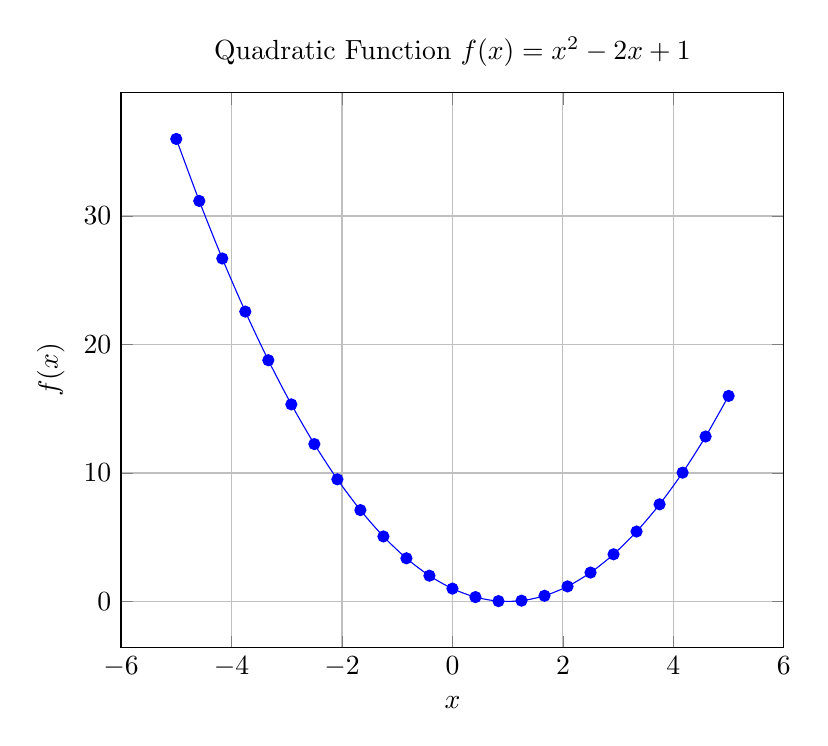
\begin{tikzpicture}
        \begin{axis}[
            xlabel={$x$},
            ylabel={$f(x)$},
            title={Quadratic Function $f(x) = x^2 - 2x + 1$},
            grid=major
        ]
        \addplot[color=blue,mark=*,smooth] {x^2 - 2*x + 1};
        \end{axis}
    \end{tikzpicture}
\end{figure}

\section{Supplementary Notes}

\begin{note}
    These notes are a personal compilation of key mathematical concepts, serving as a study aid and reference for Advanced Mathematical Analysis.
\end{note}

\begin{Problem}{Research Challenge}{prob:research}
    Investigate the convergence properties of the series $\sum_{n=1}^{\infty} \frac{1}{n^p}$ for different values of $p$.
\end{Problem}

\end{document}
